Collecting data is nothing new. Information is gathered in the form of samples, or collections of observations. Samples are collected from populations, which are collections of all individuals or individual items of a particular type. At times a population signifies a scientific system; other times it is represented as the rest of society. When conducting a data analysis, we aim to identify relationships in society, in other words, to estimate the parameters of the population. While collecting data is one step, analysing it and drawing meaningful conclusions is a much more complex task. To help make these decisions and draw conclusions, inferential statistics are used. Specifically, fitting a regression model to data based on a sample and making predictions based on the model about the population. \newline

\noindent The central problem when regression models are fitted to data is to determine the true relationship among the variables. The problem is that the true relationship is not known, and we have to depend upon the sample observations to estimate the true relationship. In this case, the chosen regression model should be able to generalise beyond the sample data. \newline 



\subsection{Assumptions for Regression Models}

\noindent Regression models are tools for understanding relationships between variables. However, for this to work, certain assumptions need to be satisfied. This section will briefly explain the previously mentioned key assumptions that are essential to ensure reliable results and the ability to predict beyond the sample. It is still possible to create regression models without these assumptions, but it becomes undeniably harder.  \newline

\noindent The first assumption is called Independence of Errors, and it states that the errors from the model are not correlated with each other, they are independent. This means that one error cannot be used to predict the next one. \newline


\noindent The next is the assumption of Linearity, which states that the relationship between the independent variables and the parameters, also known as the coefficients, is linear. This does not mean that the regression model itself has to be linear. For example, in polynomial regression, the relationship between the independent variables and the coefficients is still linear, but the independent variables can be transformed using powers.\newline


\noindent Then there is Homoscedasticity, which is the assumption of constant variance across errors for all levels of the independent variables. This assumption will be addressed in more detail later. \newline

\noindent Next, is the assumption, Normality of Errors which states that the errors between the model and the observed values, also called residuals, are normally distributed. If this is not met, it may result in a biased model and a worse model fit. \newline


\noindent Then, there is also the assumption of Multicollinearity which occurs when two or more independent variables in a regression model are highly correlated with each other. This means that changes in one independent variable are associated with changes in another, making it difficult to determine the individual effect of each independent variable on the dependent variable. \newline

\noindent Last assumption is Correct Model Specifications which assume that the provided dependent variables for the models are the correct ones. If one is missing, or the model is overfitting, this may result in incorrect coefficients and introduce errors into the model. \newline

\noindent These assumptions are not guaranteed when working with empirical data, which could make the results inaccurate. 
If such a case occurs, there are different ways to accommodate the situation. These methods will be further discussed later on. \newline 

 

\subsection{Empirical Data}
To give an example of a data set containing assumption violations is the "Miles Per Gallon" data set. Through the "Miles Per Gallon" it's possible to model the violations in the assumptions, as seen in \autoref{fig:1} and \autoref{fig:2}.
\newline

\begin{figure}
	\centering
	\centering
	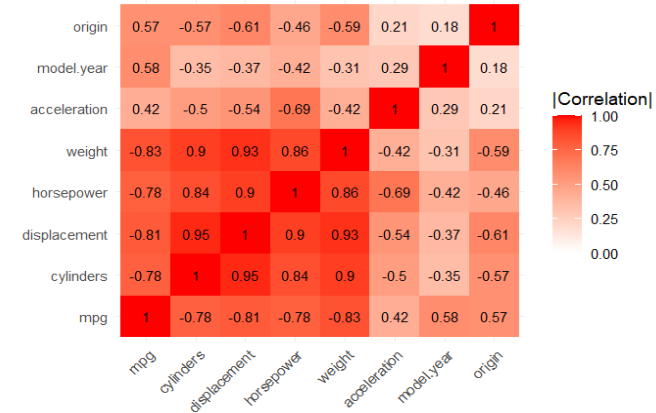
\includegraphics{billder/1.png}
	\caption{Heatmap made from the MPG dataset}
	\label{fig:1}
\end{figure}

\noindent Multicollinearity can be seen in Figure 1. Multicollinearit occurs when independent variables are highly correlated with each other, and as a result, it becomes more difficult to isolate the individual effect of each variable in a regression model.
In this model it is shown through the numbers, where the high numbers suggest a strong linear relationship through the variables. So between 'displacement' and ' cylinders', the value is 0.95, which is close to 1 and therefore shows there is multicollinearity.


\begin{figure}[h]
	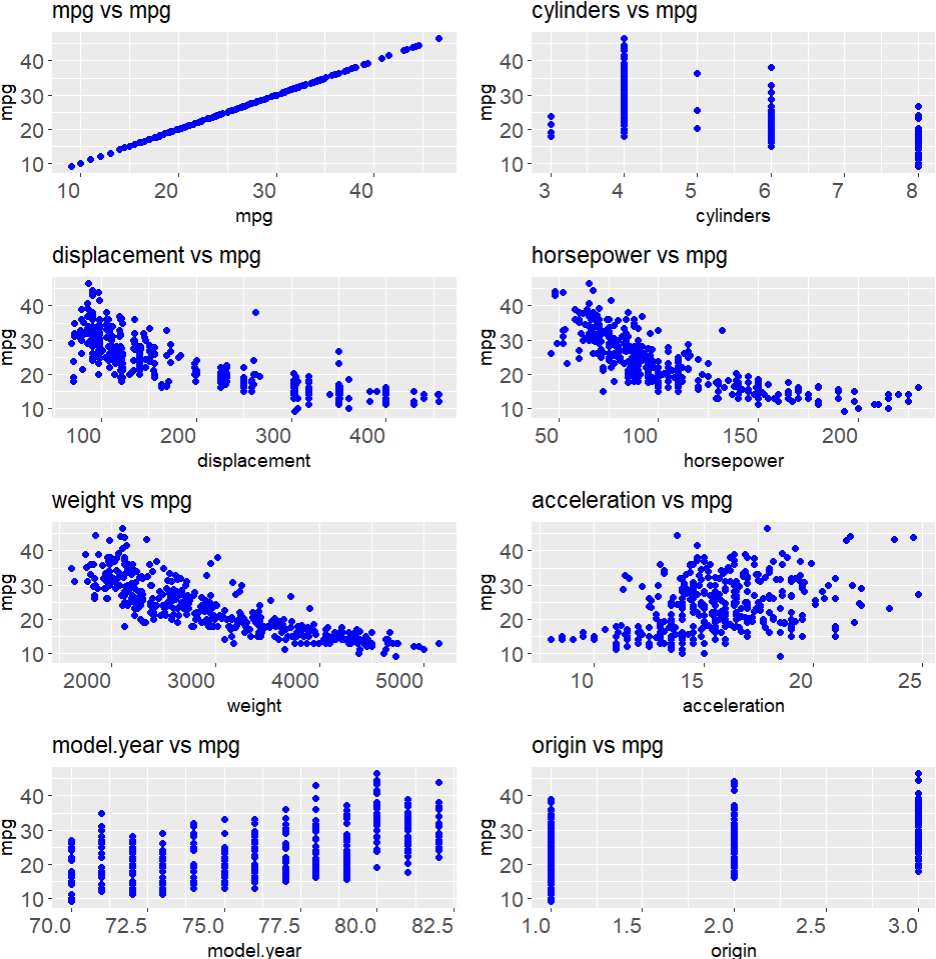
\includegraphics[width=\linewidth]{billder/2.png}
	\caption{Scatterplots made from the MPG dataset}
	\label{fig:2}
\end{figure}
\noindent There is an example of hetereoscedasticity in the 'mpg' and 'horsepower' scatterplot in Figure 2, where there is not constant variance of the residuals. This is seen because there is a big spread between the variables, especially when horsepower decreases.   

\noindent To understand how the classical method of constructing regression models and the method of using Monte Carlo Bootstrapping works, we need to dive deeper into the background. Here, we need to understand ways to not only create a model, but how to test it as well. These topics will be explained in the following section.

